\title{CW1: An Unknown Signal}
\date{\today}

\documentclass[10pt]{article}

\usepackage{graphicx}
\usepackage{parskip}

%\usepackage{minted}

\date{}

\author{Originally by: Michael Wray \& Davide Moltisanti}

\begin{document}
\maketitle

\section{Introduction}
\label{sec:intro}
The year is 1983, the strategy of D\'etente (de-escalation via verbal agreement) has failed.
Both the United States of America and the Soviet Union have been stockpiling nuclear weapons and recent political events have brought the world on the cusp of total annihilation.
As an operator for a nuclear early warning device you receive an unknown signal... 

\section{Task}
\label{sec:task}
In this coursework you will be given example points which follow an unknown signal.
You will be required to reconstruct the signal and give the resulting error.
\textbf{Your mark will be based on a report you write about the code, submitted to the ``Data-Driven Computer Science Coursework'' submission point.
You will also submit the code as a single python file to ``Code submission point''.  
We will check that the code satisfies the basic requirements (in the implementation section) and for plagarism, but we won't assess its performance. [The previous passage is highlighted from the original text. It means that in the absence of serious issues such as nonexistant/clearly nonsense implementation or plagarism, mark is 100\% driven by report.  In general, we will not be running the code, so details such as paths to files, or output format don't matter].}

You are required to work on this coursework individually. You may consult with your peers on the concepts and spirit of the assignment/solution, but you may not exchange code or passages of text for the report.

The deadline is April 30th at noon UK time.

\section{Implementation}
\label{sec:implementation}
Your final solution will use the linear least squares regression code that you have created in the worksheets which will need to be extended in order to cope with non-linear curves.
Your solution should:
\begin{itemize}
  \item Read in a file containing a number of different line segments (each made up of 20 points)
  \item Determine the function type of line segment, 
  \begin{itemize}
    \item linear
    \item polynomial with a fixed order that you must determine (same order for all segments in all files)
    \item unknown nonlinear function that you must determine (same function for all segments in all files)
  \end{itemize}
  \item Use maximum-likelihood/least squares regression to fit the function
  \item Produce the total reconstruction error 
  \item Produce a figure showing the reconstructed line from the points if an optional argument is given. 
\end{itemize}

\paragraph{Note:} All Code written for the least squares regression sections must be written by yourself.
You can use anything in the Python standard library (https://docs.python.org/3/library/) but the only external libraries your solution should use are:
\begin{itemize}
  \item Numpy
  \item Pandas
  \item Matplotlib
\end{itemize}
e.g. \texttt{scipy}, \texttt{sk\_learn} and \texttt{torch} are not permitted.

\section{Report}

The aim of this report is to demonstrate your understanding of methods you used, the results you obtained and your understanding of issues such as overfitting.
The report should be no more than 4 pages long, using no less than 11 point font, with at least 2 cm margins.
You should include:
\begin{itemize}
  \item (Briefly) equations for linear regression.
  \item Justification for your choice of polynomial order.  Include plots.
  \item Justification for your choice of unknown function.  Include plots.
  \item Description of your proceedure for selecting between linear/polynomial/unknown functions, accounting for overfitting.  Marks won't be based on the exact choice of proceedure as long as there's some attempt to deal with overfitting.  But top marks will be available for a discussing the advantages and disadvantages of your particular method.  e.g.\ does it give different answers depending on the random seed?  did you choose to make the method slightly less accurated in exchange for being faster? are there some examples where your method (or other methods you considered) fail? if so why? how much does it matter? how could we fix it?  (Please don't try to answer all of these questions, the discussion will depend alot on your proceedure and how you arrived at it).
\end{itemize}


%\section{Marks}
%\label{sec:marks}
%Each solution will go through 50 tests in order to test its correctness and robustness.
%These test files will be similar in nature to the train files that you have been provided.
%Each test will be worth 2 points broken down as the following: 
%\begin{itemize}
%    \item 0: Solution gave incorrect output format and/or didn’t finish execution. 
%    \item 1: Solution gave correct output format but a large error difference. 
%    \item 2: Solution gave correct output format and a small error difference. 
%\end{itemize}
%\paragraph{Note:} The ‘error difference’ will be the difference in error between your solution and a model solution we have coded.
%This will be different for every test and more information will be provided when the marks are released. 
%
%\subsection{Up to $40\%$}
%Solutions which have implemented the linear least squares regression.
%
%\subsection{Up to $60\%$}
%Solutions with an extended least squares regression to handle polynomial inputs with few errors.
%
%\subsection{Up to $80\%$}
%Solutions with an extended least squares regression fine-tuned to the output signal which fail on edge cases.
%
%\subsection{Up to $100\%$}
%A perfect solution that reconstructs every signal with minimum error.


\section{Train/Test Files}
\label{sec:train_files}
The input files are Comma Separated Value (CSVs) which consists of two columns for the x and y dimensions respectively.
Each input file will be split into different line segments each made up of 20 different points, so the first 20 points correspond to the first line segment, 21-40 the second line segment \textit{etc}.
Two consecutive line segments may/may not follow the same trend.
A line segment will follow a linear, polynomial or another unknown function.
An example train file is given below (basic\_2.csv): 

\begin{verbatim}
    -2.9251047704944395,4.8735802196928955
    -0.8554275589011144,8.298220787115126
    0.19855925795710938,10.042225113162727
    0.43421216060191,10.432153786922873
    0.624770694735732,10.747465992520771
    1.3614382007711343,11.96641038237006
    1.5943359027154818,12.351780097835984
    4.194060135884697,16.653475561819924
    4.6779257660237565,17.45411532191076
    5.023596843152395,18.026088181779052
    7.288865840413205,21.774369344024162
    7.485381750603618,22.099539063443302
    7.932320124145074,22.839076261125182
    9.697898711534522,25.760532815546593
    9.79296969415338,25.91784427553536
    10.338531977763036,26.820571869016863
    10.47247053028027,27.042196476913674
    11.373020960538451,28.532313640689885
    12.448760928878032,30.31231233562508
    12.518847008701732,30.428281932638267
    12.653923639452994,30.27170891389091
    12.717363846157376,30.149430959474596
    12.922893495415568,29.753282422312626
    13.82087982807715,28.02245685354787
    16.940698414027672,22.009156225167718
    17.888369346145012,20.182565974932835
    19.383541905873596,17.300692607859034
    19.669839705150725,16.748867336976346
    20.098166635136398,15.923287731535833
    20.564236539021604,15.024960354898298
    20.621376796845194,14.914825249663732
    21.505205350325678,13.211288120947877
    27.70770290983017,1.2562716850382856
    28.51062072023851,-0.2913138686887322
    28.664485990065593,-0.5878817934724623
    29.937739282405232,-3.042016420848668
    30.093442528905104,-3.3421269574788823
    30.886445731764947,-4.870602580881737
    31.512235111191547,-6.076781582919168
    31.755689686592167,-6.546028595495876
\end{verbatim}

This corresponds to 40 points of x and y co-ordinates which make up the two different line segments of the file. 
Test files could consist of any number of line segments (\textit{i.e.} longer than adv\_3.csv) as well as have large amounts of noise. 

\section{Input/Output}
\label{sec:IO}

We expect a program called \textbf{lsr.py} (\textbf{not a jupyter notebook}) which will be run as follows:
\begin{verbatim}
    $ python lsr.py basic_2.csv
\end{verbatim}

After execution your program should print out the total reconstruction error, created by summing the error for every line segment, followed by a newline character:

\begin{verbatim}
    $ python lsr.py basic_2.csv
    6.467081701001855e-27
    $
\end{verbatim}

Additionally, to further understand and validate your solution we wish for your program to be able to visualise the result given an optional parameter, \texttt{--plot}.
This is only to visually check that your solution is working (and so that you can save plots for your report).
For example, running:

\begin{verbatim}
    $ python lsr.py basic_2.csv --plot
    6.467081701001855e-27
\end{verbatim}

Will also show the following visualisation:

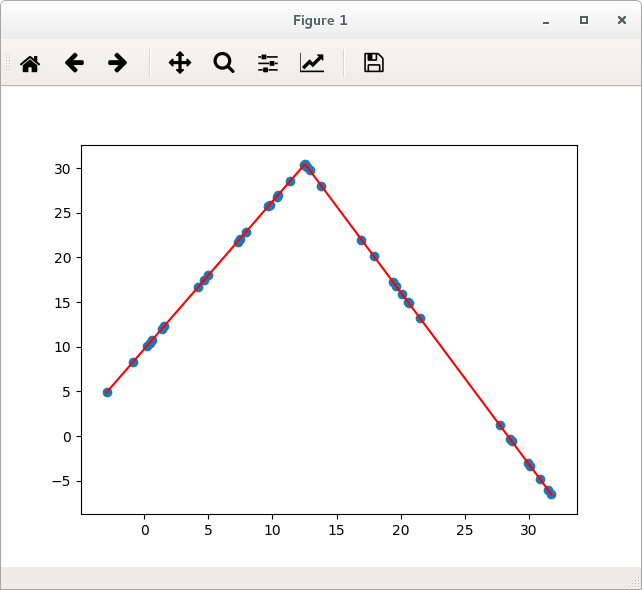
\includegraphics[width=0.65\textwidth]{CW1_visualisation}

Note the presence of both the original points (blue dots) and fitted line segments (red lines).

\section{Hints/Notes}
\label{sec:hints/notes}
\begin{itemize}
    \item We have provided you a utilities file which contains two functions: \textit{load\_points\_from\_file} and \textit{view\_data\_points}.
        The first will load the data points from a file and return them as two numpy arrays.
        The second will visualise the data points with a different colour per segment.
        Feel free to copy-paste this code into your final solution (it will be excluded from plagarism checks).
    \item The error you need to calculate is the sum squared error. 
    \item Regardless of the number of segments your program needs to only output the total reconstruction error. 
    \item The test files will include points approximating line segments generated from the three functions mentioned above, \textit{i.e.} linear, polynomial or the unknown function. 
    \item The order of the polynomial (and the form of the unknown function) \textbf{will not} change between different files/segments.
    \item Having a very low error might not be the correct answer to a noisy solution, refer to overfitting in the lecture slides. 
    \item You probably shouldn't use regularisation (the coursework is designed under the assumption that you'll use the simplest possible function classes to mitigate overfitting, rather than regularisation).
    \item In some settings (especially with noisy data), you might improve cross-validation performance by using a polynomial with a too-low order.  We're really looking for the one polynomial (remember, same across all segments in all files) that we used to generate data.  So you might find segments where using a too-low order to mitigate overfitting helps cross-validation sometimes.  (Noise-free data are your friend here).
\end{itemize}

\appendix

\section{Odd vertical offsets and the precision of matrix inversion}

In a recent Q\&A session, Peter Marsh raised the issue of strange vertical offsets when using the usual formula for linear regression, especially when using higher-order polynomials.

\includegraphics[width=0.4\textwidth]{offset.png}

Importantly, you don't actually need to address this issue to solve the CW (which is why we hadn't uncovered the issue until now; it seems to emerge mainly for a few segements and for polynomials that are higher-order than the true ones).

\textbf{Further, we only got to the bottom of these issues a week before the final deadline, so no one is going to be penalised if they don't deal with this issue (or even for including plots that look like this)! There are no marks for discussing these issues in the report (you can include it, but it will take space away from topics that will be marked).}

Matthew Nagy and Jonathan Marriott noted that this might be an issue with the numerical stability in the matrix inversion.
In particular, \texttt{np.linalg.inv} gives ever-so-slightly wrong answers, and in a few settings this can cause major issues in the plotting.
There are a few potential solutions.
\begin{itemize}
  \item Note that the $x$'s in this plot are all large and postive.  This causes all the $x$, $x^2$, $x^3$ features to be highly correlated, which can cause instabilities. To fix this, you could include an additive offset for the $x$'s (in this example subtracting $\sim 20$) to make the $x$'s roughly centered on $0$.  Note that this only works because polynomials with an additive offset in the $x$'s are still polynomials (i.e. $a x^2 + b x + c = a' (x-\theta)^2 + b' (x-\theta) + c'$).  This might not be true for the unknown function, so \textbf{don't add an x-offset when fitting the unknown function!}
  \item Use $(\mathbf{X}^T \mathbf{X} + \delta \mathbf{I})^{-1}$ rather than $(\mathbf{X}^T \mathbf{X})^{-1}$, where $\delta$ is small relative to $\mathbf{X}^T \mathbf{X}$.  The extra diagonal component should make the matrix inverse more stable.  But be careful!  This is very similar to regularisation, so may make higher-order polynomials appear to fit better.
  \item Combine the matrix-multiply and matrix-inverse operations using \texttt{np.linalg.solve} rather than \texttt{np.linalg.inv}.  This is probably the hardest to implement,because the documentation for \texttt{np.linalg.solve} isn't very good, and I can't give more details on how top use it effectively without giving away a key part of the solution.  So if you're not happy with this approach and you still need to resolve this issue, try one of the first two approaches!
\end{itemize}
As always with numerical computations, these strategies may work in some circumstances and fail in others, so always do careful testing!
And it certainly isn't the case that one of these is the ``best'' answer.

\end{document}
